\documentclass[manuscript]{acmart}

\usepackage{graphicx}
\graphicspath{{./Source/}}

\begin{document}

    \title{A Polynomial Time Algorithm for 3SAT} % Sets article title
    \author{Robert Quigley}
    % what should I do for \affiliation?
    \email{robertquigley21@gmail.com}
    % do not use \thanks for journals
    % see the acks environment sec 2.13
    % remember to put the CCS codes in!!
    
    \begin{abstract}
        This paper includes the presentation of a polynomial time algorithm to
        solve 3SAT. It begins with the problem definition and format of various
        parts of the problem. It then offers lemmas of important aspects of 
        the 3SAT problem along with their corresponding proofs. Next, it describes
        the algorithm that uses these lemmas to solve 3SAT in polynomial times. And finally, it proves
        that the algorithm works for any general case of 3SAT. The algorithm relies
        on the fact that an instance of 3SAT is unsatisfiable iff contradicting
        1-terminal clauses can be derived in polynomial time.
    \end{abstract}
    
    % TODO: google a list of keywords for ACM journals
    \keywords{test1, test2}
    
    \maketitle 

    % \acmplain for theorem, conjecture, proposition, lemma, corollary, etc
    % \acmdefinition for example and definition
    % \acks for acknowledgements
    % bibtex or biblatex for bibliography
    
    TODO: find who the heck wrote '3SAT is NP-complete'
    read https://dl.acm.org/doi/10.1145/800157.805047
    
    \section{Definitions}

    \begin{definition}
        Terminals: symbols used in the 3SAT problem that can be assigned a value
        of either 0 or 1, True or False, or any other binary assignment. They usually
        take the form $x_i$ where $i$ is a natural number.
    \end{definition}
    \begin{definition}
        Terms: terminals in either the positive or negated form. If a term is positive, 
        then the value of the terminal will be the same as the value of the term. If a
        term is negated, then the value of the terminal will be the opposite of the 
        value of the term.
    \end{definition}
    \begin{definition}
        Clauses: a set of terms combined by logical or operators.
        Clauses usually take the form 
        $(x_i \lor \neg x_j \lor x_k)$ where $x_i \neq x_j \neq x_k$
    \end{definition}
    \begin{definition}
        (3SAT) Instance: a set of any number of clauses combined by logical
        and operators. Note that entire clauses may not be negated. Terminals may
        not repeat within a clause, but they are free to repeat between clauses. 
        Instances usually take the form:
        $(x_i \lor \neg x_j \lor x_k) \land (x_l \lor x_m \lor x_n)$
    \end{definition}
    \begin{definition}
        Assignment: A list of values in which each value represents either True
        or False such that each item in the list corresponds to a terminal and 
        all terminals are assigned a value.
    \end{definition}
    \begin{definition}
        Satisfying Assignment: An assignment, $A$, is said to satisfy the instance, 
        if applying $A$ will make the instance evaluate to True.
    \end{definition}
    \begin{definition}
        The 3SAT Problem: Given a 3SAT instance, does there exist a satisfying assignment?
    \end{definition}
    \begin{definition}
        Satisfiable: an instance is satisfiable iff there exists a satisfying assignment.
    \end{definition}
    \begin{definition}
        Unsatisfiable: an instance is unsatisfiable iff there does not exist a satisfying assignment.
    \end{definition}
    \begin{definition}
        Blocking an Assignment: An assignment, $A$, is said to be blocked if, given a
        clause, $C$, there is no way that $A$ can satisfy the instance.
    \end{definition}
    \begin{definition}
        TODO: define a more 'specifically in polytime' type of implication
        Implication: A clause, $C$, is said to imply another clause, $D$, if all 
        assignments blocked by $D$ are also blocked by $C$ 
    \end{definition}
    \begin{definition}
        Given Clauses: clauses which were given in the original instance.
    \end{definition}
    \begin{definition}
        Implied Clauses: clauses which are implied by the clauses in the original instance.
    \end{definition}
    \begin{definition}
        k-terminal (k-t) clause: a clause is described as a k-terminal or a k-t clause
        if there are $k$ terminals in the clause
    \end{definition}
    \begin{definition}
        Reduction: A special type of implication in which the implied 
        clause is shorter than the implying clause(s).
    \end{definition}
    \begin{definition}
        Expansion: A special type of implication in which the 
        implied clause is longer than the implying clause(s).
    \end{definition}
    \begin{definition}
        Contradicting Clauses: A set of clauses is said to be contradicting if
        they block every assignment
    \end{definition}

    \section{Reformatting}

    Since there are a lot of constant characteristics about an instance of 3SAT, 
    we can remove most of them to allow ourselves to focus only on what changes
    from instance to instance. A list of unchanging characteristics follows:
    \begin{itemize}
        \item the symbol $x$
        \item logical and operators
        \item logical or operators
    \end{itemize}
    
    The only difference between instances, therefore, is the subscript of the terminal.
    The following items will be changed to improve compatibility with python code:
    *possible footnote to describe how to represent it as list of lists
    \begin{itemize}
        \item parentheses will become square brackets
        \item negation symbols will become minus signs
        \item an instance may be surrounded with square brackets to show it is a list of lists
    \end{itemize}
   
    For example, the instance:
    
    $(\neg x_a \lor x_b \lor x_c) \land (x_a \lor x_d \lor x_e)$

    will be written as:

    $[[-a, b, c], [a, d, e]]$


    \section{Lemmas}

    \begin{lemma}        
        For a given instance with $n$ terminals, there are $2^n$ possible assignments.
    \end{lemma}
    \begin{proof}
        An assignment for this instance consists of $n$ values, each with two possible
        values, True or False.

        Therefore, there are $2^n$ possible assignments.
    \end{proof}

    \begin{lemma}
        If a clause contains the same terminal in its negated and positive form, it will
        always be true.
    \end{lemma}
    \begin{proof}
        Given: a clause containing the same terminal in both the positive and
        negative form.

        We know that terminal must either be True or False. Consider both cases:

        That terminal's value is True:
        The positive form of the terminal will be true and the clause will evaluate to true

        That terminal's value is False:
        The negative form of the terminal will be true and the clause will evaluate to true
    \end{proof}

    \begin{lemma}
        For a given instance with $n$ terminals, there are $8 * {n \choose 3}$
        possible 3-terminal clauses that block at least one instance.
    \end{lemma}
    \begin{proof}
        Recall from Lemma 3.2 that a clause containing the same terminal in both
        the positive and negated form will always be true.

        Therefore, it will never block any assignments.

        Recall also that an instance containing the same terminal in the same
        form twice is not a valid 3SAT clause.

        Therefore we do not have to consider clauses containing the same terminal
        twice since we are concerned with clauses that block assignments.

        Given an instance with $n$ terminals, choose three of them to make a clause
        
        Once the terminals are selected, each terminal can have one of two values, either
        True or False

        There are $2 * 2 * 2$ possible clauses based on these terminals

        Since there are $8$ clauses for every selection of three terminals, there are
        $8 * {n \choose 3}$ possible clauses
    \end{proof}

    \begin{lemma}
        A clause can block an assignment    
    \end{lemma}
    \begin{proof}
        Recall the definition of a clause blocking an assignment:
        An assignment is blocked if it does not allow the clause to evaluate to True.

        Since terms in a clause are combined by logical OR operators, a 
        clause cannot evalute to True iff all terms evalute to False.

        A term evaluates to False if it's either (1) negated and the terminal's
        value is True or (2) positive and the terminal's value is False

        Given a clause, we know there are three unique terminals and we can
        find assignments where all terms evalute to False.

        This would force the clause to evalute to False.

        Since the instance is composed of clauses combined by logical AND operators 
        and one clause evalutes to False, then the entire instance evalutes to False.

        Since the instance evaluates to False, the assignment cannot satisfy
        the instance.

    \end{proof}


    \begin{lemma}
        Each assignment can be blocked by at most ${n \choose 3}$ 3-terminal clauses
    \end{lemma}
    \begin{proof}
        Consider an assignment, A. WTS it is blocked by ${n \choose 3}$ clauses.

        Recall from Lemma 3.4 that an assignment is blocked based on values of
        the three terminals in the clause blocking it.

        Notice also that each of these values only has one possible option since
        assignments have a fixed value for each terminal.

        Recall assignments are of length $n$.

        We can choose three of the $n$ values in the assignments to fix and
        make a clause out of it in the following manner:

        if the value is False, the term is positive

        if the value is True, the term is negated

        This will create a clause that blocks the assignment.

        This allows us to have ${n \choose 3}$ possible clauses that block an assignment.
        
    \end{proof}

    \begin{lemma}
        Each clause of length $k$ blocks $2^{n-k}$ assignments
    \end{lemma}
    \begin{proof}
        In this proof, I will use $a, b, c$ instead of $x_a, x_b, x_c$ and
        I will use 0 and 1 instead of False and True

        Now, consider the general k-terminal clause, $C$ in an instance with
        $n$ terminals.

        As seen in Lemma 3.4, this blocks all assignments where all of the terms evaluate to False

        Since the values for $k$ terminals are set, there are $n-k$ terminals left
        whose values could be 0 or 1.

        Since an assignment exists for every possible way to assign values to
        each terminal, we know an assignment exists for every possible way to
        assign a value for these $n-k$ terminals

        Since the values of $k$ terminals are fixed, there are $2^{n-k}$
        unique assignments that are blocked by $C$.
    \end{proof}

    \begin{lemma}
        Adding clauses to an unsatisfiable instance will never make it satisfiable.
        Similarly, removing clauses from a satisfiable instance will never make it unsatisfiable.
    \end{lemma}
    \begin{proof}
        1. Recall that clauses block assignments and an instance is unsatisfiable if
        none of the possible assignments satisfy the instance, ie, an instnace is 
        unsatifiable if all of the assignments are blocked.

        Therefore, adding clauses to an instance in which all assignments are blocked
        will never be able to unblock an assignment and it will remain unsatisfiable.

        2. An instance is satisfiable if there exists a satisfying assignment, ie, 
        an instance is satisfiable if there is at least one assignment that's not blocked.

        Therefore, removing clauses will never be able to block that assignment and
        the instance will remain satisfiable.
    \end{proof}

    \begin{lemma}
        For any clause, C, if we select a terminal, t, that's not in C then half of the assignments
        blocked by C will assign True to t and the other half will assign False to t
    \end{lemma}
    \begin{proof}
        We have a clause, C, of arbitrary length:

        [1, 2, 3, ...]

        Now we select a terminal, t, that's not in C, say we call this terminal $t$

        WTS half of the assignments blocked by C assign True to $t$ and the other half
        assign False to $t$.

        We know there will be no overlap between these assignments because a single assignment
        cannot assign both the values True and False to the same terminal.

        Now we just have to show that exactly half of the assignments are blocked by assigning
        either True or False to $t$. Let's say we assign True to $t$.

        Let's say there are $k$ terms in C, then we know it blocks assignments where
        all of the terms evaluate to False.

        By Lemma 3.6, this clause blocks $2^{n-k}$ assignments. 

        If we fix the calue of $t$ to True, then there are only $n-k-1$ terminals
        whose values could be 0 or 1. Since we have two choices per terminal
        and there are $n-k-1$ terminals, then there are $2^{n-k-1}$ assignments
        blocked by $C$ where the value of $t$ is fixed.

        Divide 
        
        $2^{n-k-1}/2^{n-k}$

        = $2^{n - k - 1 - (n - k)}$

        = $2^{-1}$

        = $1/2$

        This shows that half of the assignments blocked by $C$ assign a fixed
        value to $t$.

        Recall that a terminal can be assigned the value True or False.

        Therefore, for any clause, $C$, if we select a terminal, $t$, that's not
        in $C$ then half of the assignments blocked by $C$ will assign True
        to $t$ and the other half will assign False to $C$.

    \end{proof}

    \begin{lemma}
        Given a clause of length k, say C, all of the assignments blocked by
        another clause, say D, which contains all of the terms in C, are also blocked
        by C.
    \end{lemma}
    \begin{proof}
        Given a clause, $C$, of an arbitrary length, say $k$:

        [1, 2, 3, ...]

        And another clause, $D$, containing all the terms in $C$ with possibly
        additional terms, say of length $l$:

        [1, 2, 3, ... a, b, c, ...]

        WTS all the assignments blocked by $D$ are also blocked by $C$.

        We know that $C$ blocks all assignments that cause all the terms to evaluate
        to False.

        We know there are $2^{n-k}$ remaining terminals, each with a possible value
        of True or False.

        For each of the terminals in $D$ that are not in $C$, we know the value is fixed
        in the assignments blocked by $D$.

        Since there are $2^{n-k}$ remaining terminals, each with a possible value of True and False,
        and the assignments blocked by $D$ have set values for potentially up to the 
        rest of the terminals, all of the assignments blocked by $D$ are also blocked by $C$        
    \end{proof}

    \begin{lemma}
        Two clauses of length k that share all the same terms, except for one in which
        the same terminal is positive in one clause and negated in the other, implies
        a clause of length k-1 which is composed of all the shared terminals.
    \end{lemma}
    \begin{proof}
        Given clauses consistent with the description:

        A := [1, 2, 3, ... i]
        B := [1, 2, 3, ..., -i]

        where 1, 2, 3, ... is shared between the clauses and i is a terminal not in
        1, 2, 3, ...

        Recall that the same terminal cannot appear twice within the same clause.

        Consider the clause

        C := [1, 2, 3, ...]

        We know by Lemma 3.8 that if we select a terminal that's not in $C$, say $t$, 
        then half of the assignments blocked by $C$ assign True to $t$ and the other
        half of the assignments blocked by $C$ assign False to $t$

        Let this terminal $t$ that's not in $C$ be the terminal $i$ that's in $A$ and $B$

        We know that $A$ blocks all assignments blocked by $C$ where $i$ is assigned
        the value of 0.

        We know that $B$ blocks all assignments blocked by $C$ where $i$ is assigned
        the value of 1.

        Since $A$ and $B$ both block mutually exclusive halves of $C$, we can
        say that $A$ and $B$ imply $C$.

    \end{proof}

    \begin{lemma}
        Given a clause, C, and a terminal, t, that's not in C, two new clauses
        can be implied consisting of all the terms of C appended to either 
        the positive form of t or the negated form of t.
    \end{lemma}
    \begin{proof}
        Given a clause, C, and a terminal, t, that's not in C:

        C := [a, b, c, ...]

        By Lemma 3.8, half of the assignments blocked by $C$ assign True to $t$
        and the other half of the assignments blocked by $C$ assign False to $t$.

        We can compose two new clauses:

        D := [a, b, c, ..., t]

        E := [a, b, c, ..., -t]

        Since D and E both contain all the terminals from C, by Lemma 3.9 then
        D and E are implied by C.
        
    \end{proof}

    \begin{lemma}[Stronger Lemma 3.10]
        If two clauses have the same terminal, $t$, such that $t$ is positive
        in one clause and negated in the other, then these clauses imply a new
        clause which is composed of all the terms in both clauses that do not 
        have $t$.
    \end{lemma}
    \begin{proof}
        Consider two clauses, 

        C := [1, 2, 3, ..., t]

        D := [a, b, c, ..., -t]

        Where within a clause, the same terminal does not repeat, but between
        clauses the same terminal can repeat.

        WTS we can make a clause like this:

        E := [1, 2, 3, ..., a, b, c, ...]

        Let's define some additional clauses:

        E' := [1, 2, 3, ..., a, b, c, ..., t]

        E'' := [1, 2, 3, ..., a, b, c, ..., -t]

        % By Lemma 3.9, we know that all the clauses that C or D blocks are also
        % blocked by C' and D' respectively.

        % By Lemma 3.8, if we take any terminal, $i$, that's not in a clause, $F$, then
        % half of the assignments blocked by $F$ will assign True to $i$ and the other
        % half will assign the value False to $i$.

        By Lemma 3.9, we know that C implies E', ie, all assignments blocked by
        C are also blocked by E.

        By Lemma 3.9, we know that D implies E''.

        By Lemma 3.10, since E' and E'' share all the same terms except for t, which
        is positive in one clause and negated in the other, we can create a new
        clause composed of all the shared terms in E' and E''.

        Such a clause is already defined as E.

        Now there are a couple extra cases to consider:
        
        \begin{itemize}
            \item There is some overlap between 1, 2, 3, ... and a, b, c, ...
            \item There is the same terminal that's positive in 1, 2, 3, ... and negated in a, b, c, ...
        \end{itemize}

        First, if the same term exists in 1, 2, 3, ... and a, b, c, ..., then we
        can just remove one of the duplicates since one term being true implies an identical term being True

        Secondly, if the same terminal exists, but is of the opposite form in 1, 2, 3, ... and a, b, c, ...
        then by Lemma 3.2, this clause will always be True and thus blocks no assignments so 
        C and D do not imply E, but this type of clause is worthless so we can simply discard it.

    \end{proof}

    \begin{lemma}
        Given two clauses of length k and l that share a terminal, t, which is 
        positive in one clause and negated in the other, you will be able
        to directly imply clauses of length max(k, l)-1 to (k + l - 2)
    \end{lemma}
    \begin{proof}
        The smallest clause that can be implied by clauses of length k and l
        occur when all of the terms in one clause exist in the other.

        As such, the unique terms will come from the clause that's longer.

        Removing t, you are left with 1 less than the maximum of k and l.

        The largest clause can be implied if there are no terms shared between
        the two clauses. In this case you subtract 1 from the length of each
        clause to remove t and since no duplicates will be removed, the 
        resulting clause's length is 2 less than the sum of the lengths of 
        the clauses.
    \end{proof}

    \begin{lemma}
        Given an instance of 3SAT, you can expand all of the given clauses
        to the point where you are considering clauses of length n.
    \end{lemma}
    \begin{proof}
        TODO: PROVE
    \end{proof}

    \begin{lemma}
        If you expand given 3-t clauses as described in 3.14, you will derive
        $2^n$ unique clauses of length n iff the instance is unsatisfiable.
    \end{lemma}
    \begin{proof}
        TODO: PROVE
    \end{proof}

    \begin{lemma}
        Using the algo, 
        \begin{itemize}
            \item A 1-terminal clause can only be derived by a 2-t clause.
            \item A 2-t clause can only be derived by a 2-t or 3-t clause.
            \item A 3-t clause can only be derived by a 3-t or 4-t clause.
        \end{itemize}
    \end{lemma}
    \begin{proof}
        TODO Prove
    \end{proof}

    \begin{lemma}
        % Using the algo, if two 3-t clauses, $T_{1,2}$, are used to derive a 4-t clause, $F$,
        % then any 3-t clause, $T_3$ directly implied by $F_1$ and another 4-t
        % clause, $F_2$, are directly implied by the 3-t clauses that imply
        % the 4-t clauses.
        Given four clauses of length k - 1, A, B, C, and D, and one clause of 
        length k, E, such that 
        \begin{itemize}
            \item A and B imply E
            \item C and E imply D
        \end{itemize}
        Then A, B, and C, imply D without having to process a clause of length k
    \end{lemma}
    \begin{proof}
        Given an implied clause of length k, say C:

        [1, 2, 3, ...]

        By the algorithm, it requires two clauses to imply another clause.
        Let's call these clauses D and E. The lengths of D and E can be:

        D: length k
        
        E: length $\geq$ 2

        or

        D: length k + 1
        
        E: length any

        Okay.

        C, along with another clause, F of length m, can imply clauses of the following length:

        \begin{itemize}
            \item if k $>$ m, [k-1, k+m-2]
            \item if m $>$ k, [m-1, k+m-2] 
        \end{itemize}

        Let the clause implied by C and F be called G.
        
        Half of the assignments blocked by C are blocked by D and the 
        other half are blocked by E.

        Half of the assignments blocked by G are blocked by C and the
        other half are blocked by F.

        WTS some combo of D, E, and F, imply G.

        D + E

        D + F

        E + F

        Known:
        \begin{itemize}
            \item All terms in C exist in either D or E
            \item D and E contain an opposite term, say i
            \item All terms in D or E that's not i exist in C
            \item F must contain an opposite term from C
            \item F must contain an opposite term from D or E that's not i 
            \item D + F can imply another clause, say H
            \item E + F can imply another clause, say I
            \item H and I can derive G
        \end{itemize}
        
        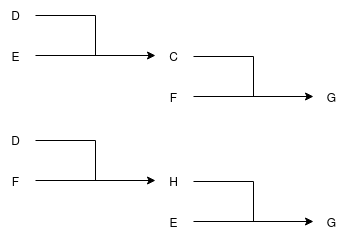
\includegraphics[scale=0.8]{317}

        Define the clauses in the following manner:

        D := [a, b, ..., i]

        E := [c, d, ... -i]

        C := [a, b, ..., c, d, ...]

        F := [-a, e, f, ...]

        G := [b..., c, d, ..., e, f, ...]

        H := [b, ..., i, e, f, ...]

        Define lengths for the ... after b, d, and f

        ... after b: $\beta$
        
        ... after d: $\delta$

        ... after f: $\phi$

        We know C is of length k and G is of length k - 1 or k.

        Let lowercase alphabetical letters represent that terminal with a count of 1

        Let letters in parentheses represent the count of terminals in both sets

        Let length of G be k

        k = a + b + $\beta$ + c + d + $\delta$ - $(\beta \delta)$ (by clause C)

        k = b + c + d + e + f + $\beta + \delta + \phi - (\beta \delta) - 
        (\beta \phi) - (\delta \phi) + (\beta \delta \phi)$ (by clause G)

        len(H) = b + i + e + f + $\beta + \phi - (\beta \phi)$

        len(H) $<$ k

        b + i + e + f + $\beta + \phi - (\beta \phi)$ $<$ 
        b + c + d + e + f + $\beta + \delta + \phi - (\beta \delta) - 
        (\beta \phi) - (\delta \phi) + (\beta \delta \phi)$

        $\rightarrow$ i + $\beta + \phi - (\beta \phi)$ $<$ 
        c + d + $\beta + \delta + \phi - (\beta \delta) - 
        (\beta \phi) - (\delta \phi) + (\beta \delta \phi)$

        $\rightarrow$ i $<$ 
        c + d + $\delta - (\beta \delta) - (\delta \phi) + (\beta \delta \phi)$

        By Venn Diagram shenanigans, $\delta - (\beta \delta) - (\delta \phi) + (\beta \delta \phi)$, 
        represents the number of terminals in $\delta$ not in $\beta$ or $\phi$

        The lowest case for the right hand side of the equation is where this is 0, ie, 
        all of the terminals in $\delta$ are in $\beta$ or $\phi$. In this case, the equation becomes:

        $\rightarrow$ i $<$ c + d

        which is guaranteed to be true since c and d both appear in E, they have to be different
        so the length of H will always be less than k, so you do not have to process
        clauses of length k to get the same implications.

        However, you may have to process clauses up to length k - 1.

        Let length of G be k - 1

        This would imply $\rightarrow$ i $<$ c + d - 1

        Alas this does not hold, so we get

        $\rightarrow$ i $=$ c + d - 1

        Which means the length of H will be k - 1, which is still shorter than C, 
        but is it short enough?

        This is only valuable if D, E, and F are of length k - 1 because then 
        this shows you will not have to process clauses of length k to
        get implications that that clause + another clause of length k - 1 will
        imply.
        
        This proves that if we have four 3-t clauses, A, B, C, and D, and one
        4-t clause, E st A and B -> E and C and E imply D, then A, B, and
        C will imply D without having to process a 4-terminal clause.

    \end{proof}

    \begin{lemma}
        Given the following clauses:
        \begin{itemize}
            \item A, of length shorter than k
            \item B, of length k
            \item C, of length shorter than k
            \item D, of length k or k - 1
            \item A expands to imply B
            \item B and C imply D
        \end{itemize}
        Then A and C can imply D by processing clauses of at most length k - 1
    \end{lemma}
    \begin{proof}

        Consider the following case:

        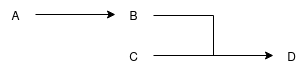
\includegraphics{318}

        A := [a, b, ...]

        B := [a, b, ..., c, d, ...]

        $C_1$ := [-a, e, f, ...]

        $C_2$ := [-c, e, f, ...]

        $D_1$ := [b, ..., c, d, ..., e, f, ...]

        $D_2$ := [a, b, ..., d, ..., e, f, ...]

        E := [b, ..., e, f, ...]

        A' := [a, b, ..., c]

        F := [a, b, ..., e, f, ...]

        Where C has to contain an opposite terminal that's either in A or not in A

        Define the following:

        $\beta$ := set of terminals after b
        $\delta$ := set of terminals after d
        $\phi$ := set of terminals after f

        Consider $C_1$ and $D_1$

        Notice A and $C_1$ share an opposite term

        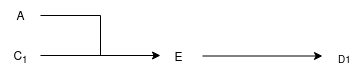
\includegraphics[scale=0.8]{318b.png}
        
        Since B is of length k, we know 

        $k = a + b + c + d + \beta + \delta - \beta \delta$

        Consider D is of length k

        $k = b + c + d + e + f + \beta + \delta + \phi - \beta \delta 
        - \beta \phi - \delta \phi + \beta \delta \phi$

        WTS length of E is less than k

        len(E) = $b + e + f + \beta + \phi - \beta \phi$

        len(E) $<$ k

        $b + e + f + \beta + \phi - \beta \phi < b + c + d + e + f + \beta + \delta + \phi - \beta \delta 
        - \beta \phi - \delta \phi + \beta \delta \phi$

        $\rightarrow 0 < c + d + \delta - \beta \delta 
        - \delta \phi + \beta \delta \phi$

        $\delta - \beta \delta - \delta \phi + \beta \delta \phi$ represents
        the number of terminals in $\delta$ not in $\beta$ or $\phi$. The lowest
        this value can be is 0.

        $\rightarrow 0 < c + d$

        This is always true, so len(E) is indeed less than k

        Consider D is of length k - 1

        Add a $-1$ to the inequality:

        $b + e + f + \beta + \phi - \beta \phi < b + c + d + e + f + \beta + \delta + \phi - \beta \delta 
        - \beta \phi - \delta \phi + \beta \delta \phi - 1$

        $\rightarrow 0 < c + d - 1$

        Which is again always true since c and d have to be different because
        they exist in the same clause, so len(E) is indeed less than k.

        Since expanding a clause only directly implies clauses of length 1 greater, 
        you only have to process clauses of length 1 shorter than D to get D

        Consider $C_2$ and $D_2$

        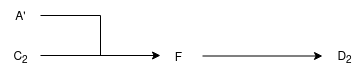
\includegraphics[scale=0.8]{318c.png}
        
        WTS A' and F are shorter than k

        Consider D is of length k

        $k = b + c + d + e + f + \beta + \delta + \phi - \beta \delta 
        - \beta \phi - \delta \phi + \beta \delta \phi$

        len(A') = $a + b + \beta + c$

        len(A') $<$ k

        $\rightarrow$ $a + b + \beta + c$ $<$ $b + c + d + e + f + \beta + \delta + \phi - \beta \delta 
        - \beta \phi - \delta \phi + \beta \delta \phi$

        $\rightarrow$ $a$ $<$ $d + e + f + \delta + \phi - \beta \delta 
        - \beta \phi - \delta \phi + \beta \delta \phi$

        In the smallest case for the R.H.S., d overlaps with e or f. 
        $\delta + \phi - \beta \delta - \beta \phi - \delta \phi + \beta \delta \phi$
        represents the number of terminals in $\delta$ + $\phi$ - overlap.
        The smallest value for this is when $\delta = \phi$

        $\rightarrow$ $a$ $<$ $e + f + \delta$

        Which is true as long as there are at least two terminals in $e, f, \delta$ or $\phi$

        Consider D is of length k - 1

        Similarly as before, we will derive

        $\rightarrow$ $a$ $<$ $e + f + \delta - 1$

        Which is true as long as there are at least three terminals in $e, f, \delta$ or $\phi$

        WTS F is shorter than k

        len(F) = $a + b + e + f + \beta + \phi - \beta \phi$

        len(F) $<$ k

        $a + b + e + f + \beta + \phi - \beta \phi$ $< $ $b + c + d + e + f + \beta + \delta + \phi - \beta \delta 
        - \beta \phi - \delta \phi + \beta \delta \phi$

        $\rightarrow$ $a$ $< $ $c + d + \delta - \beta \delta - \delta \phi + \beta \delta \phi$

        Where $\delta - \beta \delta - \delta \phi + \beta \delta \phi$ represents
        the terminals in $\delta$ that are not in $\beta$ or $\phi$

        Which is true if there are at least two terminals spread across c, d, or ($\delta$ and not $\beta$ and not $\phi$)

        Which translates to at least two terminals in $D_2$ that are not in A or $C_2$

    \end{proof}

    \begin{lemma}
        Using Lemma 3.12, a 1-t clause can only be directly implied by two 2-t clauses sharing
        the same terminal with the other terminal positive in one clause and 
        negated in the other.
    \end{lemma}
    \begin{proof}
        Given a 1-t clause, 
        
        [i]

        WTS that it can only be directly implied by 2-t clauses like 

        [i, j]

        [i, -j]

        By Lemma 3.13, the smallest clause that can be derived from two
        clauses of length k and l is max(k, l) - 1.

        With k = l = 2, this gives us a clause of length 1.

        If we increase by the lowest possible amount, say k = 3, l = 2, this
        gives us a clause of length 2.

        So we have to use two clauses of length 2 if we want to directly imply
        a clause of length 1 by using the algorithm.

        By the algorithm, both clauses must share the same terminal, where it's 
        positive in one clause and negative in the other.

        Now each clause has one remaining terminal and they could either be (1)
        the same terminal or (2) different terminals.

        \begin{enumerate}
            \item The same term:
            
            By Lemma 3.12 or more directly Lemma 3.10, this will derive a 1-t clause
            
            \item Different term:
            
            By Lemma 3.12, this will derive a 2-t clause
        \end{enumerate}

        Therefore, using Lemma 3.12, a 1-t clause can only be directly implied by 
        two 2-t clauses sharing the same terminal with the other terminal positive
        in one clause and negated in the other.

    \end{proof}

    \begin{lemma}
        The n-terminal clauses described in Lemma 3.14 can be reduced to derive
        any pair of contradicting 1-terminal clauses.
    \end{lemma}
    \begin{proof}
        TODO Prove
    \end{proof}

    \begin{lemma}
        Contradicting 1-terminal clauses can be expanded to imply
        every possible 3-terminal clause.
    \end{lemma}
    \begin{proof}
        Let the following clauses be a pair of contradicting 1-t clauses:

        [a]

        [-a]

        Let the following be a generic 3-terminal clause we want to derive
        using the contradicting 1-t clauses:

        [b, c, d]

        By Lemma 3.9, we know the 1-terminal clauses imply the following 3-t clauses:

        [a, b, c]

        [-a, b, d]

        By Lemma 3.12, these clauses imply:

        [b, c, d]
    \end{proof}

    \begin{lemma}
        Any unsatifiable instance can be converted to a form such that if one 3-terminal
        clause is removed, the instance will be satisfiable.
    \end{lemma}
    \begin{proof}
        TODO Prove    
    \end{proof}

    \begin{lemma}
        
    \end{lemma}
    \begin{proof}
        
    \end{proof}

    \begin{lemma}
        Maybe dumb but: Given an instance of 3SAT, we can add another terminal, $x_i$, 
        then for each clause, we create two new 4-terminal clauses with either form of $x_i$
        appended to the current clause.
    \end{lemma}
    \begin{proof}
        Given:

        [1, 2, 3], [1, -2, 3], [-4, -5, 6], ...

        We can add the terminal, A, and create the 4-t clauses

        [1, 2, 3, A], [1, 2, 3, -A], 
    
        [1, -2, 3, A], [1, -2, 3, -A],

        [-4, -5, 6, A], [-4, -5, 6, -A], 

        ...

        Then what do we do? I guess we want to show [[A], [-A]] exists iff the instance is unsat idk

    \end{proof}

    \begin{lemma}
        All of the clauses implied by Lemma 3.12 are all of the clauses that could possibly be implied
    \end{lemma}
    \begin{proof}
        "possibly be implied" - what does this mean?

        WTS the given clauses of length 3 can be processed to gain all of the 
        possible clauses of length 3 that are implied

        again, what does "implied" mean? are you relying on the definition of
        "imply" in your algorithm?

        WTS an unsatisfiable instance implies contradicting 1-t clauses. 

        Unsatisfiable -> all assignments are blocked

        Contradicting 1-t clauses -> 2-t clauses

        2-t clauses -> 2-t or 3-t clauses

        3-t clauses -> 3-t clauses or 4-t clauses, but all my homies hate 4-t clauses

        Proving this is another million dollar proof
    \end{proof}

    \begin{lemma}
        An instance is unsatifiable iff contradicting 1-terminal clauses can 
        be derived using the algorithm from the Algorithm section.
    \end{lemma}
    \begin{proof}
        TODO Prove the million dollar proof
    \end{proof}

    \section{Algorithm}

    \begin{enumerate}
        \item For each clause in the instance, C, of length 3 or less:
        \begin{enumerate}
            % \item Get all clauses implied by C according to Lemma 3.12
            \item For each clause in the instance, D, of length 3 or less:
            \begin{enumerate}
                \item Get all clauses implied by C and D according to Lemma 3.12 and add them to the instance
            \end{enumerate}
            \item For each clause in the instance, E, of length 1:
            \begin{enumerate}
                \item For each clause in the instance, F, of length 1:
                \begin{enumerate}
                    \item if E and F contain the same terminal in which it is 
                    positive in one clause and negated in the other, the 
                    clauses are contradicting and the instance is unsatisfiable, end
                \end{enumerate}
            \end{enumerate}
        \end{enumerate}
        \item Repeat (1) until no new clauses are added
        \item If it reaches here, the instance is satisfiable, end
    \end{enumerate}

    \section{Time Complexity Analysis}

    In this section I will analyze the time complexity of the algorithm in section 4

    (1) At most ${n \choose 3}*8 + {n \choose 2}*4 + {n \choose 2}*2$ clauses to iterate which is on the order of

    $O(n^3)$

    (1.a) At most ${n \choose 3}*8 + {n \choose 2}*4 + {n \choose 2}*2$ clauses to iterate which is on the order of

    $O(n^3)$

    (1.a.i) For each terminal in C, check if it's opposite form is in D

    $O(3^2)$ which is just constant time which is on the order of 

    $O(1)$

    (1.b) At most ${n \choose 1} * 2$ clauses of length 1 exist, which is on the order of

    $O(n)$

    (1.b.i) At most ${n \choose 1} * 2$ clauses of length 1 exist, which is on the order of

    $O(n)$

    (1.b.i.A) Constant time to check if two 1-terminal clauses contain the same terminal in the opposite form

    $O(1)$

    (2) Worst case, we add one new clause each time so we have to do (1) ${n \choose 3} * 8 + {n \choose 2} * 8 + {n \choose 1} * 2$ which is on the order of

    $O(n^3)$

    (3) Constant time to check and return satisfiable

    $O(1)$

    The time complexity breaks down:

    $(2) * ((1) * ((1.a) * ((1.a.i)) + (1.b) * ((1.b.i) * (1.b.i.A)))) + (3)$

    $= O(n^3) * (O(n^3) * (O(n^3) * (O(1)) + O(n) * (O(n) * O(1)))) + O(1)$

    $= O(n^3) * (O(n^3) * (O(n^3) * (O(1)) + O(n) * O(n))) + O(1)$

    $= O(n^3) * (O(n^3) * (O(n^3) * (O(1)) + O(n^2))) + O(1)$

    $= O(n^3) * (O(n^3) * (O(n^3) + O(n^2))) + O(1)$

    $= O(n^3) * (O(n^3) * O(n^3)) + O(1)$

    $= O(n^3) * O(n^6) + O(1)$

    $= O(n^9) + O(1)$

    $= O(n^9)$

    \section{Proof of Correctness}

    By Lemma 3.18/Lemma 3.17, if we can derive a clause of length k, say C, then
    any clause of length k - 1, say D, can be implied by 
    the clauses implying C without the need to process a clause of length 
    k or greater.

    Now, WTS an unsatisfiable instance means we will imply contradicting 1-t clauses.

    Given an unsatisfiable instance, we can expand the 3-t clauses to produce
    all possible n-terminal clauses.

    These n-terminal clauses imply clauses of length n or n-1 using the algo.

    They cannot imply any new n-terminal clauses since we already have all possible
    n-terminal clauses since it's unsatisfiable.

    And by Lemma 3.18, the n-1-terminal clauses that are implied can be implied
    without having to process clauses longer than n - 1.

    Now we have all the n-1-terminal clauses. These imply clauses between
    lengths n-2 and 2(n-1) - 2 by Lemma 3.13.

    We already have the clauses longer than n-1 so we really only care about
    implying the clauses of length n-2. 

    Again by Lemma 3.18, these clauses can be implied without having to
    process clauses greater than length n-2.

    Continue this pattern...

    We already have the clauses of length n-w and we already derived any clause
    longer than n-w so the only clauses left are the clauses of length n-w-1.
    By Lemma 3.18/Lemma 3.17, we can derive the clauses of length n-w-1 without
    processing clauses longer than n-w-1.

    Continue ...

    We already have clauses of length 4 and we already derived any clause greater
    than length 4 so the only clauses left to imply are those of length 3.
    By Lemma 3.18/3.17, we can derive the clauses of length 3 without processing
    clauses greater than length 3. 

    Now we have all the clauses of length 3, and clearly a path exists to derive
    contradicting 1-terminal clauses.

    And since we do not have to process clauses of length greater than 3, the 
    time complexity analysis in section 5 holds and it is indeed polynomial time.

    But wait! What if we get the retort: 
    Consider "we already have all clauses of length 3, doesn't Lemma 3.17/18 mean
    any 2-terminal clause implied by these can already be implied without 
    processing a clause of length 3?"
    No, because the given 3-terminal clauses were not derived, so some processing
    does have to happen.


    \section{Conclusion} 

    In this paper, we present an algorithm to solve 3SAT in polynomial time.

    By the Cook-Levin theorem, 3SAT is NP-complete, meaning 3SAT is at least
    as hard as every problem in NP.
    
    Since we have an algorithm to solve 3SAT in polynomial time, then all problems
    in NP can be solved in polynomial time.

    Thus, the class of problems, P, that can be solved in polynomial time is
    equivalent to the class of problems, NP, that can be solved in non-deterministic
    polynomial time.


    TODO:
    \begin{itemize}
        \item reorder definitions
        \item redo Lemma 3.18
        \item Perhaps modify the algo to use expansion or add another lemma
        to say 'expansion is equivalent to the current algo if we only deal with
        1-, 2-, 3-, terminal clauses'
    \end{itemize}


\end{document} 